\documentclass[a4paper, 14pt]{article}
\usepackage[margin=1.6cm]{geometry}
\usepackage[utf8]{inputenc}
\usepackage{minted}
\usepackage[russian]{babel}
\usepackage{amsmath}
\usepackage{graphicx}
\usepackage{changepage}
\usepackage{hyperref}
\usepackage{cases}
\pagestyle{empty}

\hypersetup{
	linkbordercolor = {1 1 1}
}

\usepackage[usenames,dvipsnames,svgnames,table]{xcolor}
\usepackage{tikz-timing}[2009/05/15]
\usepackage{multicol}
\usepackage[T2A]{fontenc}
\usepackage{pgfplots}
%\usepackage[left=2.5cm, right=1.5cm, vmargin=2.5cm]{geometry}
\setlength\parindent{0pt} % Удалить отступы из параграфов.

\usepackage{listings}
\usepackage{caption}
\DeclareCaptionFont{white}{\color{white}} % Текст заголовка.
\DeclareCaptionFormat{listing}{\colorbox{gray}{\parbox{\textwidth}{#1#2#3}}}
\captionsetup[lstlisting]{format=listing,labelfont=white,textfont=white}
\renewcommand\labelenumi{\theenumi)}



\begin{document}
\lstset{
	language=java,                 % Выбор языка для подсветки (здесь это java).
	basicstyle=\small\sffamily,    % Размер и начертание шрифта для подсветки кода.
	numbers=left,                  % Где поставить нумерацию строк (слева\справа).
	numberstyle=\tiny,             % Размер шрифта для номеров строк.
	stepnumber=1,                  % Размер шага между двумя номерами строк.
	firstnumber=1,
	numberfirstline=true
	numbersep=5pt,                 % Как далеко отстоят номера строк от подсвечиваемого кода.
	backgroundcolor=\color{white}, % Цвет фона подсветки - используем \usepackage{color}.
	showspaces=false,              % Показывать или нет пробелы специальными отступами.
	showstringspaces=false,        % Показывать или нет пробелы в строках.
	showtabs=false,                % Показывать или нет табуляцию в строках.
	frame=single,                  % Рисовать рамку вокруг кода.
	tabsize=2,                     % Размер табуляции по умолчанию равен 2 пробелам.
	captionpos=t,                  % Позиция заголовка вверху [t] или внизу [b].
	breaklines=true,               % Автоматически переносить строки (да\нет).
	breakatwhitespace=false,       % Переносить строки только если есть пробел.
	escapeinside={\%*}{*)}         % Если нужно добавить комментарии в коде.
}

\begin{titlepage}
	\center

	ФЕДЕРАЛЬНОЕ ГОСУДАРСТВЕННОЕ АВТОНОМНОЕ ОБРАЗОВАТЕЛЬНОЕ УЧРЕЖДЕНИЕ ВЫСШЕГО ОБРАЗОВАНИЯ\linebreak
	«Санкт-Петербургский политехнический университет Петра Великого»\\[2cm]
	\textsc{\Large Институт компьютерных наук и технологий}\\[6.5cm]

	{ \huge \bfseries КУРСОВАЯ РАБОТА	\\
	\Large \mdseries МОДЕЛИРОВАНИЕ СИСТЕМЫ, ФОРМАЛИЗОВАННОЙ КАК СИСТЕМА МАССОВОГО ОБСЛУЖИВАНИЯ \\
	\large по дисциплине <<Архитектура программных систем>>}\\[6.5cm]


	\begin{multicols}{2}
		\begin{flushright} \large

			{Выполнил студент группы: 3530904/00104:}\\[0.5cm]

			{Преподаватель:\\}

		\end{flushright}
		\begin{flushright}

			{Почернин В. С.}\\[0.5cm]


			Смирнов Н. Г.

		\end{flushright}
	\end{multicols}

	\flushright{
		{\today}\\[0.5cm]
	}
	\centering{
		Санкт-Петербург\\
		2022
	}

	\vfill
\end{titlepage}

\large
\tableofcontents
\newpage


\section{Введение}

Целью настоящей курсовой работы является построение модели системы массового обслуживания, описывающей процессы так, как они проходили бы в действительности. Модель должна описывать компоненты ВС на некотором уровне детализации, который будет имитировать её структуру и функциональность.

Модель должна давать приближенное описание объекта исследования с целью получения требуемых результатов с определенной точностью и достоверностью, принимая во внимание каждый реальный объект системы, обладающий большой сложностью и множеством состояний, связей и анализируемых характеристик.

Существуют различные типы моделей, однако в настоящей работе будет использоваться имитационная модель - логическо-математическое описание объекта, которое может быть использовано для экспериментирования на компьютере в целях проектирования, анализа и оценки функционирования объекта.

По результатам работы будет представлена оптимальная конфигурация исследуемой ВС, полученная на основе анализа экспериментов, поставленных над моделью.

\section{Первый этап}


\subsection{Бланк задания с заполненными исходными данными к работе}

\subsubsection{Вариант задания}
ИБ-ИЗ2-ПЗ1-Д10З1-Д10О3-Д2П2-Д2Б2-ОР1-ОД1

\subsubsection{Источники}
\begin{itemize}
	\item ИБ - бесконечный источник.
	\item ИЗ2 - равномерный закон распределения.
\end{itemize}

\subsubsection{Приборы}
\begin{itemize}
	\item ПЗ1 - экспоненциальный закон распределения времени обслуживания.
\end{itemize}

\subsubsection{Описание дисциплин постановки и выбора}
\begin{itemize}
	\item Д10З1 - относительный приоритет на обслуживание - запись в буфер, если есть место по кольцу.
	\item Д1003 - дисциплина отказа - самая старая в буфере.
\end{itemize}

\subsubsection{Дисциплины постановки на обслуживание}
\begin{itemize}
	\item Д2Б2 - принцип выбора заявки из буфера LIFO.
	\item Д2П2 - выбор прибора по кольцу.
\end{itemize}

\subsubsection{Виды отображения результатов работы программной модели}
\begin{itemize}
	\item ОД1 - отображение динамики функционирования модели: календарь событий, буфер и текущее состояние.
	\item ОР1 - отображение результатов: сводная таблица результатов.
\end{itemize}


\subsection{Формализованная схема ВС}
Для освоения функционирования СМО, рассмотрим формализованную схему её работы:
\begin{figure}[H]
	\centering
	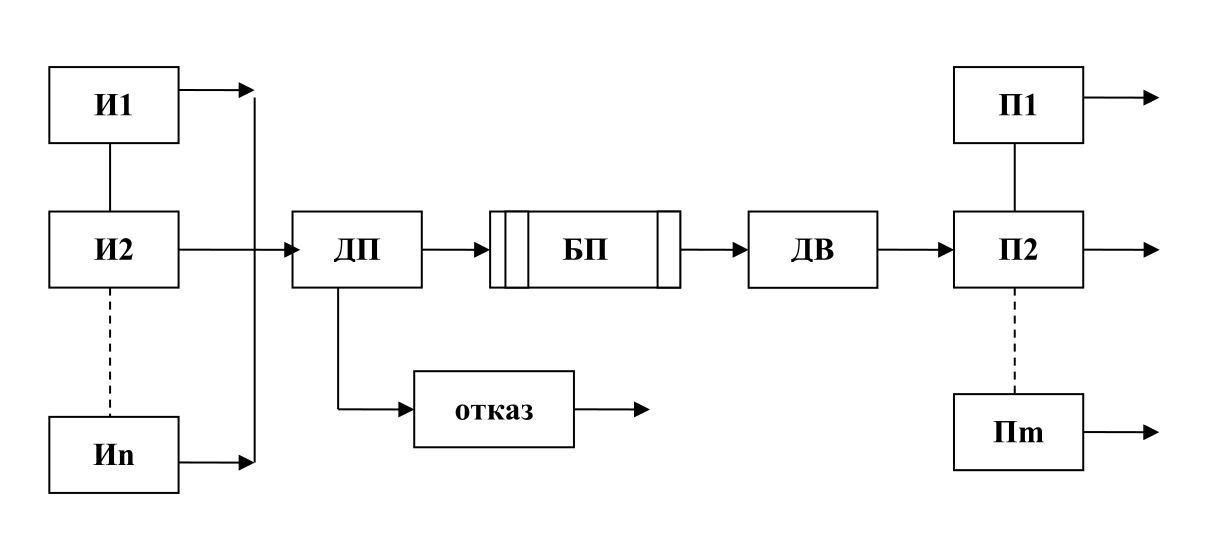
\includegraphics[width=15cm,height=\textheight,keepaspectratio]{smo.png}\\
	\caption{Формализованная схема ВС}
\end{figure}

\begin{itemize}
	\item Иi ($i=1..n$) представляют собой источники заявок, которые генерируют заявки. Все n источников вместе образуют входной поток заявок.
	\item Заявки, сгенерированные в источниках попадают на ДП - диспетчер постановки заявок в очередь. Он организует отказ или выбивание заявки из БП, если в буфере не осталось свободных мест, либо же отправляет заявку на обслуживание или в буферную память в случае отсутствия свободных приборов.
	\item БП - буферная память (место для хранения очереди заявок),  в которой хранятся заявки от различных источников.
	\item ДВ - диспетчер выбора заявок из очереди отправляет заявку из буфера на свободный прибор.
	\item П - приборы, которые обслуживают заявки и создают тем самым выходной поток заявок после обслуживания.
\end{itemize}

На основе этого, мы можем проследить путь заявки, вошедшей в модель системы:
\begin{enumerate}
	\item Постановка заявки в буфер.
	\item Отказ или выбивание (удаление) заявки из переполненного буфера.
	\item Выбор заявки из БП на обслуживание.
	\item Поиск свободного прибора.
	\item Обслуживание заявки прибором.
	\item Выход заявки из СМО.
\end{enumerate}
При этом, вся логика прохождения заявок по системе определяется диспетчерами ДП и ДВ, когда источники и приборы их только генерируют и обслуживают соответственно.


\subsection{Временная диаграмма своего варианта}
Рассмотрим временную диаграмму функционирования системы, на которой покажем
\begin{itemize}
	\item Моменты постановки заявок на приборы.
	\item Заполнение буферной памяти по заданной дисциплине постановки заявки в буфер.
	\item Отказ заявке или выбивание её при отсутствии свободных мест в БП.
	\item Функционирование дисциплины выбора заявок из буфера и дисциплины выбора приборов.
\end{itemize}
Пусть наша система будет состоять из 3 источников (И1, И2, И3), 3 позиций в буфере (Б1, Б2, Б3) и 3 приборов (П1, П2, П3). Получим следующую диаграмму:

\begin{tikztimingtable}
	И1 				& L G L L L L L L L L L L G L L L L L L L L L L L L L L L L L L L\\
	И2 				& L L L G L L L L L L G L L L L G L L L L L L L L L L L L L L L L L\\
	И3 				& L L L L L G L L G L L L L L L L L L L L L L L L L L L L L L L L\\
	П1 				& L 14D{1} 15D{2}\\
	П2 				& L L L 12D{2} L L 13D{1}\\
	П3 				& L L L L L 10D{3} L L L L 11D{2}\\
	Б1 				& L G L L L L L L G L L L L L L G L L G L L L L L L L L L L L L L L L\\
	Б2 				& L L L G L L L L L L G L L L L L L L L L L G L L L L L L L L L L L\\
	Б3 				& L L L L L G L L L L L L G L L L L L L G L L L L L L L L L L L L L\\
	\\
	Постановка      & L G L L G L L G L L G L L G L L G L L G L L L L L L L L L L L L L L L L L\\
	Изъятие         & L G L L G L L G L L L L L L L L L L G L L G L L G L L L L L L L L L L L\\
	\extracode
	\tablerules
	\begin{pgfonlayer}{background}
	\end{pgfonlayer}
\end{tikztimingtable}

\begin{itemize}
	\item Вначале мы видим, как 3 заявки поочереди создаются на источниках с первого по третий и, проходя через буфер (заходя туда по кольцу), моментально оказываются на приборах (куда они также попадают по кольцу).
	\item Затем, опять по правилу кольца, заявки с источников 3, 2 и 1 попадают на буферы 1, 2 и 3, в то время, как первые 3 заявки продолжают обрабатываться приборами, следовательно, у нас происходит заполнение буферной памяти.
	\item Внезапно, источник И2 генерирует еще одну заявку, но в буфере уже заполнены места, поэтому, приходится применять дисциплину отказа - самая старая в буфере. Заявка в буфере Б1 от источника И3, являясь самой старой, выбивается из буфера новоиспеченной заявкой от И2.
	\item Далее, по стечению обстоятельств, все три прибора одновременно заканчивают работу над своими заявками, благодаря чему мы можем увидеть работу дисциплин выбора заявок из буфера и выбора приборов. Так, как мы имеем выбор из буфера LIFO, сначала пойдет заявка с Б1, затем с Б3 и только потом Б2. Приборы же, продолжая выбираться по кольцу, возьмут заявки в порядке П1, П2, П3, так как последним прибором, взявшим заявку был П3.
\end{itemize}

\newpage

\subsection{Ответы на контрольные вопросы}

\begin{enumerate}
	\item Назовите типы источников, опишите принципы их работы, различия между ними.

	      \textbf{Ответ:} Источники бывают двух типов: бесконечные и конечные.

	      Бесконечные источники генерируют заявка, после чего определяют (по определенному закону) интервал для генерации следующей заявки. Заявка попадает в систему в момент генерации и проходит по ней свой индивидуальный путь.

	      В конечных источниках в определенный момент генерируется и отправляется в систему пакет заявок (из конечного числа заявок). Каждая заявка проходит свой индивидуальный путь по системе. Следующий пакет от такого источника генерируется тогда, когда последняя заявка из предыдущего пакета удаляется из системы (в результате обслуживания или отказа). Момент генерации определяется случайным интервалом между пакетами и новый пакет состоит из того же количества заявок.
	\item Можно ли сказать, что бесконечный источник есть частный случай конечного?

	      \textbf{Ответ:} Как мне кажется, мы не можем назвать бесконечный источник частным случаем конечного. Действительно, мы можем считать одну заявку пакетом размера 1, однако случае конечного источника мы имеем четкое условие: "Момент генерации следующего пакета определяется событием, когда последняя заявка этого пакета удаляется из системы". В случае эе бесконечного источника следующая заявка может сгенерироваться в любой момент времени, в том числе тогда, когда предыдущая заявка еще находится в системе.
	\item Опишите два принципа построения моделирующего алгоритма, их преимущества и недостатки.

	      \textbf{Ответ:} Существуют два подхода к построению моделирующего алгоритма ВС: подход Дельта-Т и подход особых событий.

	      Подход Дельта-Т является универсальным методом построения моделирующего алгоритма, в котором состояние объекта проверяется через фиксированный интервал времени. Каждый момент времени $t_i=t_{i-1}+\Delta{t_{i-1}}$ мы получаем приближенные значения характеристик исследуемого объекта. Сам промежуток $\Delta{t}$ должен быть настолько мал, чтобы не пропустить событие в моделирующей системе, которое должно быть учтено при выбранной детальности моделирования. Метод удобен тем, что он является универсальным, однако, есть и недостаток: при его использовании постоянно проверяется состояние объектов моделирования, не изменяющихся при особо малых $\Delta{t}$, что делает метод неэффективным.

	      Подход особых событий мы руководствуемся тем, что интервалы времени, в которых состояние не меняется не представляют для нас интереса. Только значимые (изменяющие состояние) переходы системы имеют для нас значение. Они определяются особыми состояниями или событиями, например:
	      \begin{itemize}
		      \item Поступление заявки в СМО (момент генерации заявки источником).
		      \item Освобождение прибора (готовность прибора взять заявку на обслуживание).
		      \item Окончание процесса моделирование, т. е. момент прекращения генерации заявок источниками.
	      \end{itemize}
	      Достоинством является эффективность данного принципа, из-за чего именно он используется в настоящей работе. К недостаткам же можно отнести сопутствующую сложность отслеживания вышеприведенных событий.
	\item Опишите дисциплины буферизации и постановки заявки на обслуживание, заданные в вашем варианте.

	      \textbf{Ответ:} в моем варианте дисциплинами буферизации являются Д10З1 - запись в буфер, если есть место по кольцу и Д1003 - дисциплина отказа - самая старая в буфере. Дисциплинами постановки заявки на обслуживание являются Д2Б2 - принцип выбора заявки из буфера LIFO и Д2П2 - выбор прибора по кольцу. Рассмотрим каждую из них.

	      \begin{itemize}
		      \item Д1031 - запись в буфер, если есть место по кольцу. При такой дисциплине поиск свободного места в буфере осуществляется, начиная с номера места, следующего за последним занятым. В случае, если указатель, который ищет свободное места его не найдет - начнет действовать дисциплина, организующая отказ или выбивание заявки из БП.
		      \item Д1003 - дисциплина отказа - самая старая в буфере. Эта дисциплина рассматривает только время прихода заявок в систему (момент генерации заявок источником). Заявка, раньше других вставшая в буфер получает отказ, уходит из системы и на её место встает пришедшая заявка.
		      \item Д2Б2 - принцип выбора заявки из буфера LIFO (последним пришел - первым обслужен). В этом лсучае раньше других будет выбрана из буфера та заявка, которая пришла последней.
		      \item Д2П2 - выбор прибора по кольцу. Поиск свободных приборов здесь каждый раз начинается с указателя и заявка встает на обслуживание в первый из найденных приборов.
	      \end{itemize}
	\item Назовите некоторые варианты (комбинации) значений входных параметров, при которых на представленной временной диаграмме могут появиться отказы из БП и будут хорошо проиллюстрированы дисциплины выбора приборов и выбора заявок.

	      \textbf{Ответ:} отказы из БП могут появиться тогда и только тогда, когда любой из источников генерирует заявку в то время, как буфер находится в заполненном состоянии. Например, мы получили 6 заявок от источников, 3 отправились на приборы, 3 в буфер (который после этого заполнился). Генерируется 7-я заявка, которой нет места в буфере, из-за чего применяется дисциплина отказа.

	      Выбор заявок можно явно увидеть, если, например, заполнить по очереди весь буфер и заметить, что забираться заявка будет в обратном порядке. Это покажет нам, что буфер работает как стек, то есть по правилу LIFO.

	      Что касается приборов, мы можем заметить их выбор по кольцу в самом начале, когда они начнут по очереди заполняться заявками. Если же затем приборы одновременно закончат обрабатывать заявки, то новыми заявками они начнут заполняться в том же порядке, поскольку указатель кольца начнет с первого прибора (так как последним прибором был последний прибор в кольце).
\end{enumerate}

\section{Второй этап}

\subsection{Описание}

В рамках второго этапа необходимо разраблтать и отдалить программу, которая смоделирует поведение текущей ВС.



\subsubsection{Отражение работы программной модели}

В текущем задании предусмотрены два вида отражения работы программной модели:
\begin{itemize}
	\item Отображение \textbf{динамики} функционирования модели в \textbf{пошаговом} режиме.
	\item Отображение \textbf{результатов} работы программной модели в \textbf{автоматическом} режиме.
\end{itemize}

\paragraph{Динамика в пошаговом режиме}

Здесь нужно отразить изменение состояние ВС при каждом наступлении особого события.

Фиксация осуществляется пошагово, где \textbf{шаг} - расстояние по времени от одного особого события до ближайшего другого.

В текущем задании необходимо отразить работу программной модели в пошаговом режиме в виде \textbf{календаря событий} (календарь событий, буфер, текущее состояние).

Данная функциональность будет реализована посредством четырех частей:

\begin{itemize}
	\item Кнопки перехода вперед/назад/на конкретный шаг.
	\item Текстовое описание текущего шага.
	\item Таблица календарь событий/текущее состояние:
	      \begin{center}
		      \begin{tabular}{|c|c|c|c|}
			      \hline
			      \multicolumn{2}{|c|}{Календарь событий} & Число заявок & Число отказов   \\
			      \hline
			      Событие                                 & Время        &               & \\
			      \hline
			      И1                                      &              &               & \\
			      \hline
			      ...                                     &              &               & \\
			      \hline
			      Иm                                      &              &               & \\
			      \hline
			      П1                                      &              &               & \\
			      \hline
			      ...                                     &              &               & \\
			      \hline
			      Пk                                      &              &               & \\
			      \hline
			      Конец мод.                              &              &               & \\
			      \hline
		      \end{tabular}
	      \end{center}
	      \begin{itemize}
		      \item Событие - наименование описываемого элемента.
		      \item Время - абсолютное время очередного события (например, время, когда источник сгенерирует заявку или когда прибор обработает заявку).
		      \item Число заявок - число созданных (в случае источника) или обслуженных (в случае прибора) заявок на данный момент.
		      \item Число отказов - количество отказов на данный момент.
	      \end{itemize}
	\item Таблица буфер:
	      \begin{center}
		      \begin{tabular}{|c|c|c|c|}
			      \hline
			      Позиция & Время постановки & Источник & Заявка \\
			      \hline
			      1       &                  &          &        \\
			      \hline
			      ...     &                  &          &        \\
			      \hline
			      N       &                  &          &        \\
			      \hline
		      \end{tabular}
	      \end{center}
\end{itemize}

\paragraph{Результаты в автоматическом режиме}

Для представления результатов моделирования в автоматическом режиме, в процессе работы программной модели для каждой заявки происходит сбор \textbf{статистической информации} для расчета следующих характеристик системы:

\begin{itemize}
	\item Количество заявок сгенерированных каждым источником.
	\item Вероятность отказа в обслуживании заявок каждого источника:
	      $$p=\frac{m}{n}, \quad \text{где}$$
	      \begin{itemize}
		      \item n - общее количество заявок, сгенерированных источником.
		      \item m - количество заявок этого источника, получивших отказ.
	      \end{itemize}
	\item Среднее время пребывания заявки каждого источника в системе:
	      $$T_{\text{преб}} = T_{\text{обсл}} + T_{\text{БП}}, \quad \text{где}$$
	      \begin{itemize}
		      \item $T_{\text{преб}}$ - среднее время пребывания заявки в системе (время ответа на запрос).
		      \item $T_{\text{обсл}}$ - среднее время обслуживания заявки данного источника.
		      \item $T_{\text{БП}}$ - среднее время пребывания заявки в БП или среднее время ожидания заявки каждого источника.
	      \end{itemize}
	\item Дисперсии $T_{\text{обсл}}$ и $T_{\text{БП}}$.
	\item Коэффициенты использования приборов ($\frac{\text{Суммарное время занятости каждого прибора}}{\text{Общее время реализации}}$).
\end{itemize}

Соответственно, после завершение процесса моделирования должны быть получены две таблицы результатов:

\begin{center}
	\begin{tabular}{|c|c|c|c|c|c|c|c|}
		\hline
		\multicolumn{8}{|c|}{Характеристики источников ВС}                                                                                                   \\
		\hline
		№ источника & Количество заявок & $p_\text{отк}$ & $T_\text{преб}$ & $T_\text{БП}$ & $T_\text{обсл}$ & $\text{Д}_\text{БП}$ & $\text{Д}_\text{обсл}$ \\
		\hline
		И1          &                   &                &                 &               &                 &                      &                        \\
		\hline
		И1          &                   &                &                 &               &                 &                      &                        \\
		\hline
		...         &                   &                &                 &               &                 &                      &                        \\
		\hline
		Иm          &                   &                &                 &               &                 &                      &                        \\
		\hline
	\end{tabular}
\end{center}

\begin{center}
	\begin{tabular}{|c|c|}
		\hline
		\multicolumn{2}{|c|}{Характеристики приборов ВС} \\
		\hline
		№ прибора & Коэффициент использования            \\
		\hline
		П1        &                                      \\
		\hline
		П2        &                                      \\
		\hline
		...       &                                      \\
		\hline
		Пk        &                                      \\
		\hline
	\end{tabular}
\end{center}

Отдельно стоит отметить, что \textbf{окончание процесса генерации заявок} (конец моделирования) происходит в момент \textbf{генерации последней заявки}, однако в СМО могут остаться заявки как на приборах, так и в буферной памяти, поэтому процесс \textbf{обслуживания заявок} продолжается до момента \textbf{выхода из системы последней заявки}.

\textbf{Общим временем реализации} называется время, которым заканчивается обслуживание последней заявки (именно его значение используется при расчете коэффициентов использования приборов).

\subsection{Законы распределения}

При моделировании ВС подразумевается использование двух законов распределения:
\begin{itemize}
	\item Равномерный закон распределения времени генерации для бесконечных источников.
	\item Экспоненциальный закон распределения времени обслуживания для приборов.
\end{itemize}
Рассмотрим каждый из них.

\subsubsection{Равномерный закон распределения}

Равномерный закон распределения характеризуется функцией распределения вида:

\begin{equation*}
	F(x) =
	\begin{cases}
		0,               & x < a         \\
		\frac{x-a}{b-a}, & a \le x \le b \\
		1                & x > b
	\end{cases}
\end{equation*}

Построим график распределения при $a = 22$ и $b = 55$:

\begin{tikzpicture}[
		declare function={
				func(\x,\a,\b) =
				(\x < \a) * (0) +
				and(\x >= \a,\x <= \b) * ((\x-\a) / (\b-\a)) +
				(\x>\b) * (1);
			}
	]
	\begin{axis}[
			title = Равномерный закон распределения,
			xlabel = {$x$},
			xmin=0,
			xmax=100,
			ylabel = {$F(x)$},
			minor tick num = 2
		]
		\addplot[
			color=blue,
			domain=0:100,
		]{func(x, 22, 55)};
	\end{axis}
\end{tikzpicture}

Соответственно:
\begin{equation}
	x=F(x)(b-a)+a
\end{equation}

Где $F(x)$ будет случайным числом в диапазоне от 0 до 1.

\subsubsection{Экспоненциальный закон распределения}

Экспоненциальный закон распределения характеризуется функцией распределения вида:
\begin{equation*}
	F(x) = 1 - e^{-\lambda x}
\end{equation*}

Построим график распределения при $\lambda = 3$:

\begin{tikzpicture}
	\begin{axis}[
			title = Экспоненциальный закон распределения,
			xlabel = {$x$},
			xmin=0,
			xmax=100,
			ylabel = {$F(x)$},
			minor tick num = 2
		]
		\addplot[
			color=blue,
			domain=0:100,
		] {1-e^(-0.1*x)};
	\end{axis}
\end{tikzpicture}

Соответственно:
\begin{equation}
	x = -\frac{1}{\lambda}log_e(1-F(x))
\end{equation}
Где F(x) будет случайным числом в диапазоне от 0 до 1.


\subsection{Ответы на контрольные вопросы}

\begin{enumerate}
	\item Какие изменения состояние ВС должны фиксировать программа для текущего задания в пошаговом режиме?

	      \textbf{Ответ:} Мы работаем с методом особых состояний, а значит, что для нас имеют значение только значимые (изменяющие состояние) переходы системы в некоторые моменты времени. Они будут определяться следующими состояниями или событиями:
	      \begin{itemize}
		      \item Поступление заявки в СМО (момент генерации заявки источником).
		      \item Поступление заявки в БП (либо же срабатывание отказа).
		      \item Переход заявки из буфера в свободный прибор.
		      \item Освобождение прибора (и взятие им заявки из буфера, при наличии таковых).
		      \item Окончание процесса моделирования (момент прекращения генерации заявок источниками).
		      \item Выход из системы последней заявки.
	      \end{itemize}
	\item Что должно являться шагом при работе программной модели в режиме динамического отражения результатов?

	      \textbf{Ответ:} При работе программной модели в режиме динамического отражения результатов \textbf{шаг} - это интервал модельного времени от одного особого события до другого ближайшего по времени особого события.
	\item Из чего складывается время пребывания заявки в системе и как рассчитывать среднее время пребывания заявки в системе?.

	      \textbf{Ответ:} Время пребывания заявки в системе рассчитывается по следующей формуле:
	      $$T_{\text{преб}} = T_{\text{обсл}} + T_{\text{БП}}, \quad \text{где}$$
	      \begin{itemize}
		      \item $T_{\text{преб}}$ - среднее время пребывания заявки в системе (время ответа на запрос).
		      \item $T_{\text{обсл}}$ - среднее время обслуживания заявки данного источника.
		      \item $T_{\text{БП}}$ - среднее время пребывания заявки в БП или среднее время ожидания заявки каждого источника.
	      \end{itemize}
	      Чтобы рассчитать именно \textbf{среднее} время - будем для каждого источника суммировать времена заявок и их количество, а затем возьмем среднее арифметическое.
	\item Как рассчитать коэффициент использования приборов $K_{\text{исп}}$?

	      \textbf{Ответ:} $\text{Коэффициент использования приборов} = \frac{\text{Суммарное время занятости каждого прибора}}{\text{Общее время реализации}}$.
	\item В чем разница между окончанием моделирования и общим временем реализации?

	      \textbf{Ответ:}
	      \begin{itemize}
		      \item \textbf{Окончание процесса моделирования} (конец моделирования, окончание процесса генерации заявок) происходит в момент \textbf{генерации последней заявки}, но в этот момент в СМО еще могут оставаться заявки как на приборах, так и в буферной памяти.
		      \item \textbf{Общее время реализации} - это время, которым заканчивается обслуживание последней заявки. То есть момент выхода из системы последней заявки.
	      \end{itemize}
	\item Какие сведения должны быть выведены на экран по истечении времени реализации?.

	      \textbf{Ответ:} После истечения времени реализации, на экран должны быть выведены две таблицы результатов:
	      \begin{itemize}
		      \item Характеристики источников ВС.
		      \item Характеристики приборов ВС.
	      \end{itemize}
\end{enumerate}

\section{Третий этап}

\subsection{Описание}

На третьем этапе нужно привести пример потенциально-существующей ВС (реальной или гипотетической), которая бы полностью соответствовал бы дисциплинам и законам варианта задания.

Также нужно иметь достаточно четкое представление о моделируемой системе, чтобы написать количественные значения входных параметров.

В итоге, мы хотим получить выходные характеристики и сравнить их со сформулированными требованиями к результатам работы.

\subsubsection{Определение эффективности ВС}

Определять эффективность нашей ВС будем по следующим выходным характеристикам:

\begin{itemize}
	\item $p_\text{отк}$ - вероятность отказа в обслуживании заявок;
	\item $T_\text{преб}$ - среднее время пребывания заявок в СМО;
	\item $T_\text{БП}$ - среднее время пребывания заявок в буфере;
	\item $K_\text{исп}$ - коэффициент использования приборов;
\end{itemize}

Задавая желаемые количественные значения этим трём выходным характеристикам, мы формируем требования к работе создаваемой ВС.

\subsubsection{Подход к проектированию модели}

Говоря грубо, мы должны определить, что нужно подать на вход нашей модели, чтобы получить подходящие нам выходные характеристики.

Однако, комбинаций входных значений может оказаться бесконечное множество, поэтому на множество входных значений следует наложить ограничения, исходя из особенности конкретно нашей ВС.

Таким образом, получится спроектирована модель архитектуры системы, которая будет работать по заданным требованиям.

\subsection{Пример ВС, соответствующей модели}


Приведем \textbf{пример потенциально-существующей ВС}, которая бы соответствовала всем законам и дисциплинам нашей модели:


\subsubsection{Описание ВС}

\begin{itemize}
	\item Мы - отечественная сыродельная компания, которая занимается производством молодых сыров из собственного сырья.
	\item В нашем распоряжении есть коровы (источники заявок), которые поставляют нам молоко. Это молоко собирается в резервуары и отправляется на заготовку сыра в ёмкости для сырной массы (приборы).
	\item Если в настоящий момент времени у нас нет свободных емкостей для сыра, то мы отправляем резервуары с молоком на склад (буфер).
	\item Наша цель - добиться лучшего результата - соотношения потраченных денег (на коров и закваску) к количеству производимого сыра.
\end{itemize}

\subsubsection{Соответствие модели с ВС}

\begin{center}
	\begin{tabular}{|p{0.2\linewidth} | p{0.3\linewidth}| p{0.5\linewidth}|}
		\hline
		Часть системы      & Описание закона/дисциплины                                                           & Соответствие с реальной ВС                                                                                                                                                                                                                                                                                                                                                                                                                                                                                                                                                                                                                                     \\
		\hline
		Источники          & Бесконечный источник с равномерным законом распределения времени генерации заявок.   & Источники в нешй системе - это \textbf{коровы}, которые дают нам молоко. Производство молока у коровы зависит от множества факторов: её самочувствия, настроения, погоды и породы. Поэтому коровы будут давать нам молоко бесконечно с равномерным законом распределения времени между сбором. При этом, мы можем выбрать между тремя породами коров, которые имеют разное время "генерации молока".                                                                                                                                                                                                                                                           \\
		\hline
		Приборы            & Экспоненциальный закон распределения времени обслуживания заявок.                    & Приборами у нас будут \textbf{емкости для сырных масс}, в которых будут производиться наши молодые сыры. Хотя мы и специализируемся на молодых сырах - здесь тоже есть некоторый разброс по времени (очень молодой сыр, умеренно молодой сыр, итд). При этом, чаще всего мы будем производить очень молодой сыр, но иногда будем делать линейку сыров, готовящихся подольше. Этим будет объясняться экспоненциальный закон распределения времени. При производстве сыра, мы можем также выбрать один из трех вариантов: не добавлять закваску вовсе, добавить дешевую закваску или добавить дорогую закваску, что будет менять время изготовления нашего сыра. \\
		\hline
		Буфер              &                                                                                      & Буфером у нас будет \textbf{склад с резервуарами}, где будет храниться выдоенное молоко, готовящееся к превращению в сыр.                                                                                                                                                                                                                                                                                                                                                                                                                                                                                                                                      \\
		\hline
		Постановка в буфер & Запись в буфер, если есть место по кольцу.                                           & Каждый резервуар, где хранится молоко у нас не отличается от другого, и использоваться они должны \textbf{равномерно}. Здесь идеально подойдет распределение мест по кольцу.                                                                                                                                                                                                                                                                                                                                                                                                                                                                                   \\
		\hline
		Отказ в буфере     & Если при постановке в буфер в нем нет мест - из него выбивается самая старая заявка. & Если выбирать - приготовить сыр из более старого или из более нового молока - \textbf{мы всегда будем выбирать новое}, поскольку сыр в таком случае будет получаться крайне нежным. Поэтому, когда у нас появляется свежевыдоенное молоко, а места для него нет - оно будет занимать место самого старого на данны момент молока.                                                                                                                                                                                                                                                                                                                              \\
		\hline
		Выбор из буфера    & Выбор заявки по LIFO(стек).                                                          & Опять же, выбирая между старым и новым молоком, лучше выбрать новое, потому что это принесет нам больше пользы. Так как мы хотим держать планку качества, то будем пытаться \textbf{всегда выбирать самое молодое молоко} со склада.                                                                                                                                                                                                                                                                                                                                                                                                                           \\
		\hline
		Выбор прибора      & Выбор прибора по кольцу.                                                             & Как и резервуары для молока, емкости для сыра также не отличаются друг от друга и лучше всего использовать их \textbf{равномерно}, в чем нам поможет выбор прибора по кольцу.                                                                                                                                                                                                                                                                                                                                                                                                                                                                                  \\
		\hline
	\end{tabular}
\end{center}

\subsubsection{Ограничения и требуемые характеристики}

Согласно нашей системе, можно выдвинуть следующие ограничения:

\begin{itemize}
	\item \textbf{Вероятность отказа} должна составлять \textbf{не более 15\%} - мы не хотим, производимое нами молоко уходило впустую
	\item \textbf{Коэффициент использования приборов} должен быть \textbf{более 80\%} - Чем больше работают приборы - тем больше денег мы сможем заработать. Нельзя, чтобы был простой и мы бы тратились на емкости для сыра впустую.
	\item \textbf{Среднее время пребывания заявок в буфере} Среднее время пребывания заявки (резервуара с молоком) в буфере должно быть не более 5 суток, иначе качество продукции может упасть.
\end{itemize}

\begin{center}
	\begin{tabular}{|p{0.5\linewidth} | p{0.5\linewidth}|}
		\hline
		Количество источников (коров)               & от 1 до 3                                                                                                                                \\
		\hline
		Размер буфера (количество резервуаров)      & от 30 до 50                                                                                                                              \\
		\hline
		Количество приборов (емкостей для сыра)     & от 40 до 60                                                                                                                              \\
		\hline
		Скорость работы источников (коров)          & $a = 10$, $b = 12$ - коровы 1го класса \par $a = 12$, $b = 15$ - коровы 2го класса \par $a = 15$, $b = 24$ - коровы 3го класса           \\
		\hline
		Скорость работы приборов (емкостей с сыром) & $\lambda = 0.001$ - без использования закваски \par $\lambda = 0.003$ - закваска 2го класса \par $\lambda = 0.005$ - закваска 1го класса \\
		\hline
	\end{tabular}
\end{center}

\paragraph{Примечание}

\begin{itemize}
	\item Чем быстрее корова дает молоко, тем больше её стоимость.
	\item Чем лучше сыворотка, тем больше её стоимость.
	\item Единицы времени - часы.
	\item $\lambda = 0.001$ значит, что в среднем сыр будет созревать за 40 суток.
	\item $\lambda = 0.003$ значит, что в среднем сыр будет созревать за 15 суток.
	\item $\lambda = 0.005$ значит, что в среднем сыр будет созревать за 8 суток.
\end{itemize}

\subsubsection{Ответы на контрольные вопросы}

\begin{enumerate}
	\item Опишите элементы СМО для примера своего варианта ВС по следующей схеме:
	      \begin{itemize}
		      \item Источник - тип и характеристики.
		      \item Прибор - количество и характеристики.
		      \item Буфер - тип и характеристики.
		      \item Заявка - транзакция конкретного размера.
	      \end{itemize}

	      \textbf{Ответ:} указано в таблицах.
	\item Соответствуют ли случайные законы и дисциплины постановки и выбора вашей ВС законами и дисциплинами, указанными в строчке задания вашего варианта?

	      \textbf{Ответ:} да, соответствуют, указано в таблицах.
	\item Значениями каких выходных характеристик определяется качество работы системы?

	      \textbf{Ответ:}
	      Качество работы системы определяется следующими выходными характеристиками:

	      \begin{itemize}
		      \item $p_\text{отк}$ - вероятность отказа в обслуживании заявок;
		      \item $T_\text{преб}$ - среднее время пребывания заявок в СМО;
		      \item $T_\text{БП}$ - среднее время пребывания заявок в буфере;
		      \item $K_\text{исп}$ - коэффициент использования приборов;
	      \end{itemize}
	\item Составьте требования к работе ВС (значения, которые вы хотите получить для выходных характеристик)

	      \textbf{Ответ:} составлено выше.
	\item Напишите ограничения (область изменения) для всех пяти входных параметров исследуемой ВС.

	      \textbf{Ответ:} составлено выше в таблице.
\end{enumerate}

\section{Четвертый этап}

\subsection{Описание}

Последний этап посвящен исследованию работы модели ВС и выбору её оптимальной конфигурации.

Нам необходимо получить выходные характеристики системы для всевозможных конфигураций входных параметров и отсеять только те конфигурации, выходные характеристики которой будут соответствовать заданным в третьем этапе ограничениям.

В результате мы получим некоторое множество решений исследуемой системы, т.е. некоторое количество конфигураций входных параметров, которые будут соответствовать сформулированным требованиям.

Здесь же необходимо определить количество заявок, которое должно пройти по системе, чтобы выходные характеристики были получены с заданной точностью и достоверной вероятностью.

Наконец, из полученного множества решений (вариантов архитектуры ВС) нужно будет выбрать на основе анализа результатов самый оптимальный вариант системы.

\subsection{Определение оптимального числа заявок}

Для того, чтобы иметь адекватные результаты - нам необходимо выбрать оптимальное количество заявок, которое мы будем использовать в наших конфигурациях.

В рамках задания необходимо обеспечить:
\begin{itemize}
	\item \textbf{Относительную точность}: 10\%.
	\item \textbf{Доверительную вероятность}: 0.9.
\end{itemize}
Для этого нужно определить необходимое и достаточное количество заявок, которое должно быть сгенерировано источником (чем больше заявок - тем больше точностью получения выходных характеристик).

Существует \textit{связь} между:
\begin{itemize}
	\item Количеством заявок, прошедших через ВС.
	\item Относительной точностью.
	\item Доверительной вероятностью.
	\item Случайной величиной p(A) (вероятностью события A).
\end{itemize}
\begin{equation} \label{inputs-count}
	N = \frac{t_\alpha^2(1-p)}{p\delta^2} \quad \text{, где}
\end{equation}
\begin{itemize}
	\item $N$ - количество заявок, пропущенных через систему.
	\item $p$ - вероятность отказа заявкам в обслуживании.
	\item $t_\alpha$ = 1.643 для $\alpha = 0.9$.
	\item $\delta = 0.1$ - относительная точность.
\end{itemize}

У нас имеется две неизвестные величины ($N$ и $p$). Мы хотим найти $N$ - значит нужно иметь представление о $p$. Для этого произведем \textbf{пристрелку}.

\subsubsection{Пристрелка}

Алгоритм пристрелки будет следующим:

\begin{enumerate}
	\item Назначим некоторое $N_0 = 100$ и проведем с ним процесс моделирования, получив характеристики (включая $p_0$).
	\item Подставим полученные характеристики в \eqref{inputs-count}, вычислив некоторое $N_1$.
	\item Проведем с ним аналогичный процесс моделирования, получим $p_1$.
	\item Сравним $p_1$ с $p_0$:
	      \begin{enumerate}
		      \item Если $|p_0-p_1| < 0.1p_0$, то $N=100$ удовлетворяет заданной точности результатов.
		      \item Если $|p_0-p_1| \ge 0.1p_0$, то мы продолжаем процесс моделирования с новым $N_2$ и так далее до достижения заданной точности результатов.
	      \end{enumerate}
\end{enumerate}

Этот процесс был проведен для некоторого количества конфигураций.

По результатам работы программы, были получены следующие \textbf{результаты}:

\begin{itemize}
	\item В случае, когда $p \approx 0.3$, нам достаточно $N \approx 600$.
	\item В случае, когда $p \approx 0.1$, нам достаточно $N \approx 2500$.
	\item В случае, когда $p < 0.05$, число заявок $N$ может достигать 10000.
\end{itemize}

Вследствие этого было принято решение поддерживать для всех конфигураций число заявок равное:
$$N = 10000$$

\subsection{Теория для тестирования}

Итак, для создания нашей конфигурации, мы можем варьировать следующие величины:

\begin{itemize}
	\item От 1 до 3 источников (коров).
	\item От 30 до 50 ячеек буфера (резервуаров для молока).
	\item От 40 до 60 приборов (емкостей для сыра).
	\item 3 вида коров (коровы 1го класса, коровы 2го класса, коровы 3го класса).
	\item 3 вида заквасок (без закваски, закваска 2го класса, закваска 1го класса).
\end{itemize}

Если перемножить все варианты, то мы получим следующее число возможных конфигураций:
$$3 * 21 * 21 * 3 * 3 = 11907$$

Основная цель нашей компании - получение прибыли, поэтому мы будем искать ту конфигурацию, которая будет наиболее выгодна для нас. Это означает, что она должна будет принести нам \textbf{наибольшую прибыль за час}.

Мы знаем количество заявок для каждой конфигурации - это $N = 10000$. Перемножив его на $(1-p_{\text{отк}})$, мы сможем получить \textbf{количество произведенных головок сыра}:
$$N_{\text{сыра}} = N_{\text{заявок}}\times(1-p_{\text{отказа}})$$

В зависимости от того, какую закваску мы будем использовать - будет отличаться время выращивания сыра. Чем дольше выдерживается сыр, тем он дороже, следовательно, мы определим следующую цену сыра, в зависимости от закваски:

\begin{center}
	\begin{tabular}{|c|c|c|}
		\hline
		\textbf{Тип закваски}      & \textbf{Цена головки сыра P} & \textbf{Цена закваски P} \\
		\hline
		Без использования закваски & 30 000р.                     & 0р.                      \\
		\hline
		Закваска 2го класса        & 20 000р.                     & 1000 р.                  \\
		\hline
		Закваска 1го класса        & 10 000р.                     & 2000 р.                  \\
		\hline
	\end{tabular}
\end{center}

Все наше оборудование (коровы, резервуары для молока, емкости для сыра) требуют обслуживания. В табличке ниже можно увидеть формулы, по которой будет вычисляться эта стоимость.

\begin{center}
	\begin{tabular}{|c|c|}
		\hline
		\textbf{Тип оборудования} & \textbf{Цена обслуживания (р/час) S} \\
		\hline
		Коровы 1го класса         & 300 * $N_\text{коров}$               \\
		\hline
		Коровы 2го класса         & 200 * $N_\text{коров}$               \\
		\hline
		Коровы 3го класса         & 100 * $N_\text{коров}$               \\
		\hline
		Резервуар для молока      & 5 * $N_\text{резервуаров}$           \\
		\hline
		Емкость для сыра          & 10 * $N_\text{емкостей}$             \\
		\hline
	\end{tabular}
\end{center}

Соответственно, мы сможем посчитать наш \textbf{доход} в час как:
$$\text{Доход в час = } \frac{N_\text{сыра} \times (P_\text{сыра} - P_\text{закваски})}{T_\text{симуляции}}$$

Аналогично, посчитаем \textbf{расходы} в час как:
$$\text{Расход в час} = S_\text{коров} + S_\text{резервуаров} + S_\text{емкостей} + S_\text{заквасок}$$

Наконец, мы сможем посчитать \textbf{прибыль} в час как:
$$\text{Прибыль в час} = \text{Доход в час} - \text{Расход в час}$$

Именно этот параметр мы постараемся максимизировать и выберем 10 лучших (по этому параметру конфигураций).

\subsection{Тестирование}

Тестирование нашей системы происходило \textbf{следующим образом}:

\begin{enumerate}
	\item Для каждой конфигурации было проведено тестирование и получены выходные характеристики, данные были занесены в Excel-таблицу.
	\item Изначально были получены выходные характеристики для всех 11907 конфигураций.
	\item После отсеивания заявок по ограничению вероятности отказа (не более 15\%) осталось 6148 конфигураций.
	\item После отсеивания заявок по ограничению коэффициента использования приборов (не менее 80\%) осталось 2097 конфигураций.
	\item После отсеивания заявок по ограничению среднего времени пребывания в буфере (не более 5 суток) осталось 1257 заявок.
	\item К оставшимся заявкам были применены формулы вычисления нашего критерия эффективности системы (\textbf{прибыль в час}) и был произведена сортировка по убыванию этого критерия.
\end{enumerate}

Ниже можно увидеть 10 самых эффективных конфигураций:

\small
\begin{center}
	\begin{tabular}{|c|c|c|c|c|c|c|c|c|c|c|}
		\hline
		\textbf{N}  & \textbf{N ист} & \textbf{N буф} & \textbf{N приб} & \textbf{N заявок} & \textbf{a} & \textbf{b} & \textbf{Лямбда} & \textbf{Доход, р/час} & \textbf{Расход, р/час} & \textbf{Прибыль, р/час} \\ \hline
		\textbf{1}  & 2              & 33             & 60              & 10000             & 10         & 12         & 0,003           & 3530,864              & 1365                   & 2165,864                \\ \hline
		\textbf{2}  & 2              & 32             & 60              & 10000             & 10         & 12         & 0,003           & 3512,071              & 1360                   & 2152,071                \\ \hline
		\textbf{3}  & 2              & 39             & 60              & 10000             & 10         & 12         & 0,003           & 3543,956              & 1395                   & 2148,956                \\ \hline
		\textbf{4}  & 2              & 37             & 60              & 10000             & 10         & 12         & 0,003           & 3521,841              & 1385                   & 2136,841                \\ \hline
		\textbf{5}  & 2              & 37             & 59              & 10000             & 10         & 12         & 0,003           & 3496,786              & 1375                   & 2121,786                \\ \hline
		\textbf{6}  & 2              & 31             & 60              & 10000             & 10         & 12         & 0,003           & 3475,582              & 1355                   & 2120,582                \\ \hline
		\textbf{7}  & 2              & 42             & 60              & 10000             & 10         & 12         & 0,003           & 3527,819              & 1410                   & 2117,819                \\ \hline
		\textbf{8}  & 2              & 40             & 59              & 10000             & 10         & 12         & 0,003           & 3501,347              & 1390                   & 2111,347                \\ \hline
		\textbf{9}  & 2              & 30             & 60              & 10000             & 10         & 12         & 0,003           & 3458,064              & 1350                   & 2108,064                \\ \hline
		\textbf{10} & 2              & 34             & 60              & 10000             & 10         & 12         & 0,003           & 3473,689              & 1370                   & 2103,689                \\ \hline
	\end{tabular}
\end{center}
\large

Как мы можем заметить, наилучших результатов добились конфигурации, которые использовали:

\begin{itemize}
	\item 1й класс коров (самые лучшие).
	\item 2й класс закваски (средняя по скорости и по цене производимого сыра).
	\item Максимальное количество приборов.
	\item Среднее количество коров.
	\item Размер буфера, близкий к нижней границе.
\end{itemize}

Отдельно стоит отметить, что наихудшая прибыль (среди всех отсортированных конфигураций) составила 369 рублей в час. Это значит, что нам удалось улучшить нашу систему \textbf{почти в 6 раз} с помощью произведенной симуляции.

\section{Описание программы}

\subsection{Модульная структура}

Разработка программы моделирования производилась на языке \textbf{Java} с использованием среды разработки \textbf{Intellij IDEA}. Графический интерфейс был создан как веб-приложение с использованием фреймворка \textbf{Spring}.

Приложение является объектно-ориентированным и содержит следующую структуру:

\begin{enumerate}
	\item Пакет \textbf{controller} - хранит в себе контроллеры:
	\begin{enumerate}
		\item \textbf{SimulationController} - отвечает за обработку HTTP запросов графического интерфейса.
	\end{enumerate}
	\item Пакет \textbf{data} - хранит в себе дата-классы для хранения информации:
	\begin{enumerate}
		\item \textbf{BufferTableRow} - дата-класс, описывающий строку таблицы буфера.
		\item \textbf{CalendarAndStateTableRow} - дата-класс, описывающий строку таблицы календаря событий и текущего состояния.
		\item \textbf{DeviceCharacteristicTableRow} - дата-класс, описывающий строку таблицы характеристик приборов.
		\item \textbf{InputCharacteristicTableRow} - дата-класс, описывающий строку таблицы характеристик источников.
		\item \textbf{SimulationResult} - дата-класс, описывающий результаты симуляции.
		\item \textbf{StepData} - дата-класс, описывающий шаг симуляции.
	\end{enumerate}
	\item Пакет \textbf{research} - хранит в себе классы, ответственные за исследование модели:
	\begin{enumerate}
		\item \textbf{OutputCharacteristics} - дата-класс, описывающий выходные характеристики моделирования.
		\item \textbf{Sighting} - класс, ответственный за пристрелку.
		\item \textbf{Tests} - класс, ответственный за тест модели (прогон всевозможных конфигураций).
	\end{enumerate}
	\item Пакет \textbf{simlation} - хранит в себе классы, ответственные за симуляцию:
	\begin{enumerate}
		\item \textbf{Buffer} - класс, реализующий функциональность буфера.
		\item \textbf{BufferPlace} - класс, реализующий функциональность места в буфере.
		\item \textbf{Config} - класс, хранящий в себе конфигурацию системы.
		\item \textbf{Device} - класс, реализующий функциональность прибора.
		\item \textbf{DeviceKit} - класс, реализующий функциональностью набора приборов.
		\item \textbf{Event} - класс, реализующий функциональность события.
		\item \textbf{EventType} - перечисление, хранящее тип события.
		\item \textbf{Input} - класс, реализующий функциональностью источника.
		\item \textbf{InputKit} - класс, реализующий функциональностью набора источников.
		\item \textbf{Request} - класс, реализующий функциональностью заявки.
		\item \textbf{Simulation} - класс, ответственный за симуляцию.
	\end{enumerate}
	\item Пакет \textbf{utils} - хранит в себе вспомогательные классы.
	\begin{enumerate}
		\item \textbf{Utils} - класс, хранящий вспомогательные методы (получение распределений времени).
	\end{enumerate}
\end{enumerate}

\subsection{Демонстрация работы программы}

Так как у нас написано веб-приложение - программа запускается в браузере. По умолчанию это происходит по адресу \textit{http://localhost:8080/}.

При переходе по данному адресу открывается главная страница:

\begin{figure}[H]
	\centering
	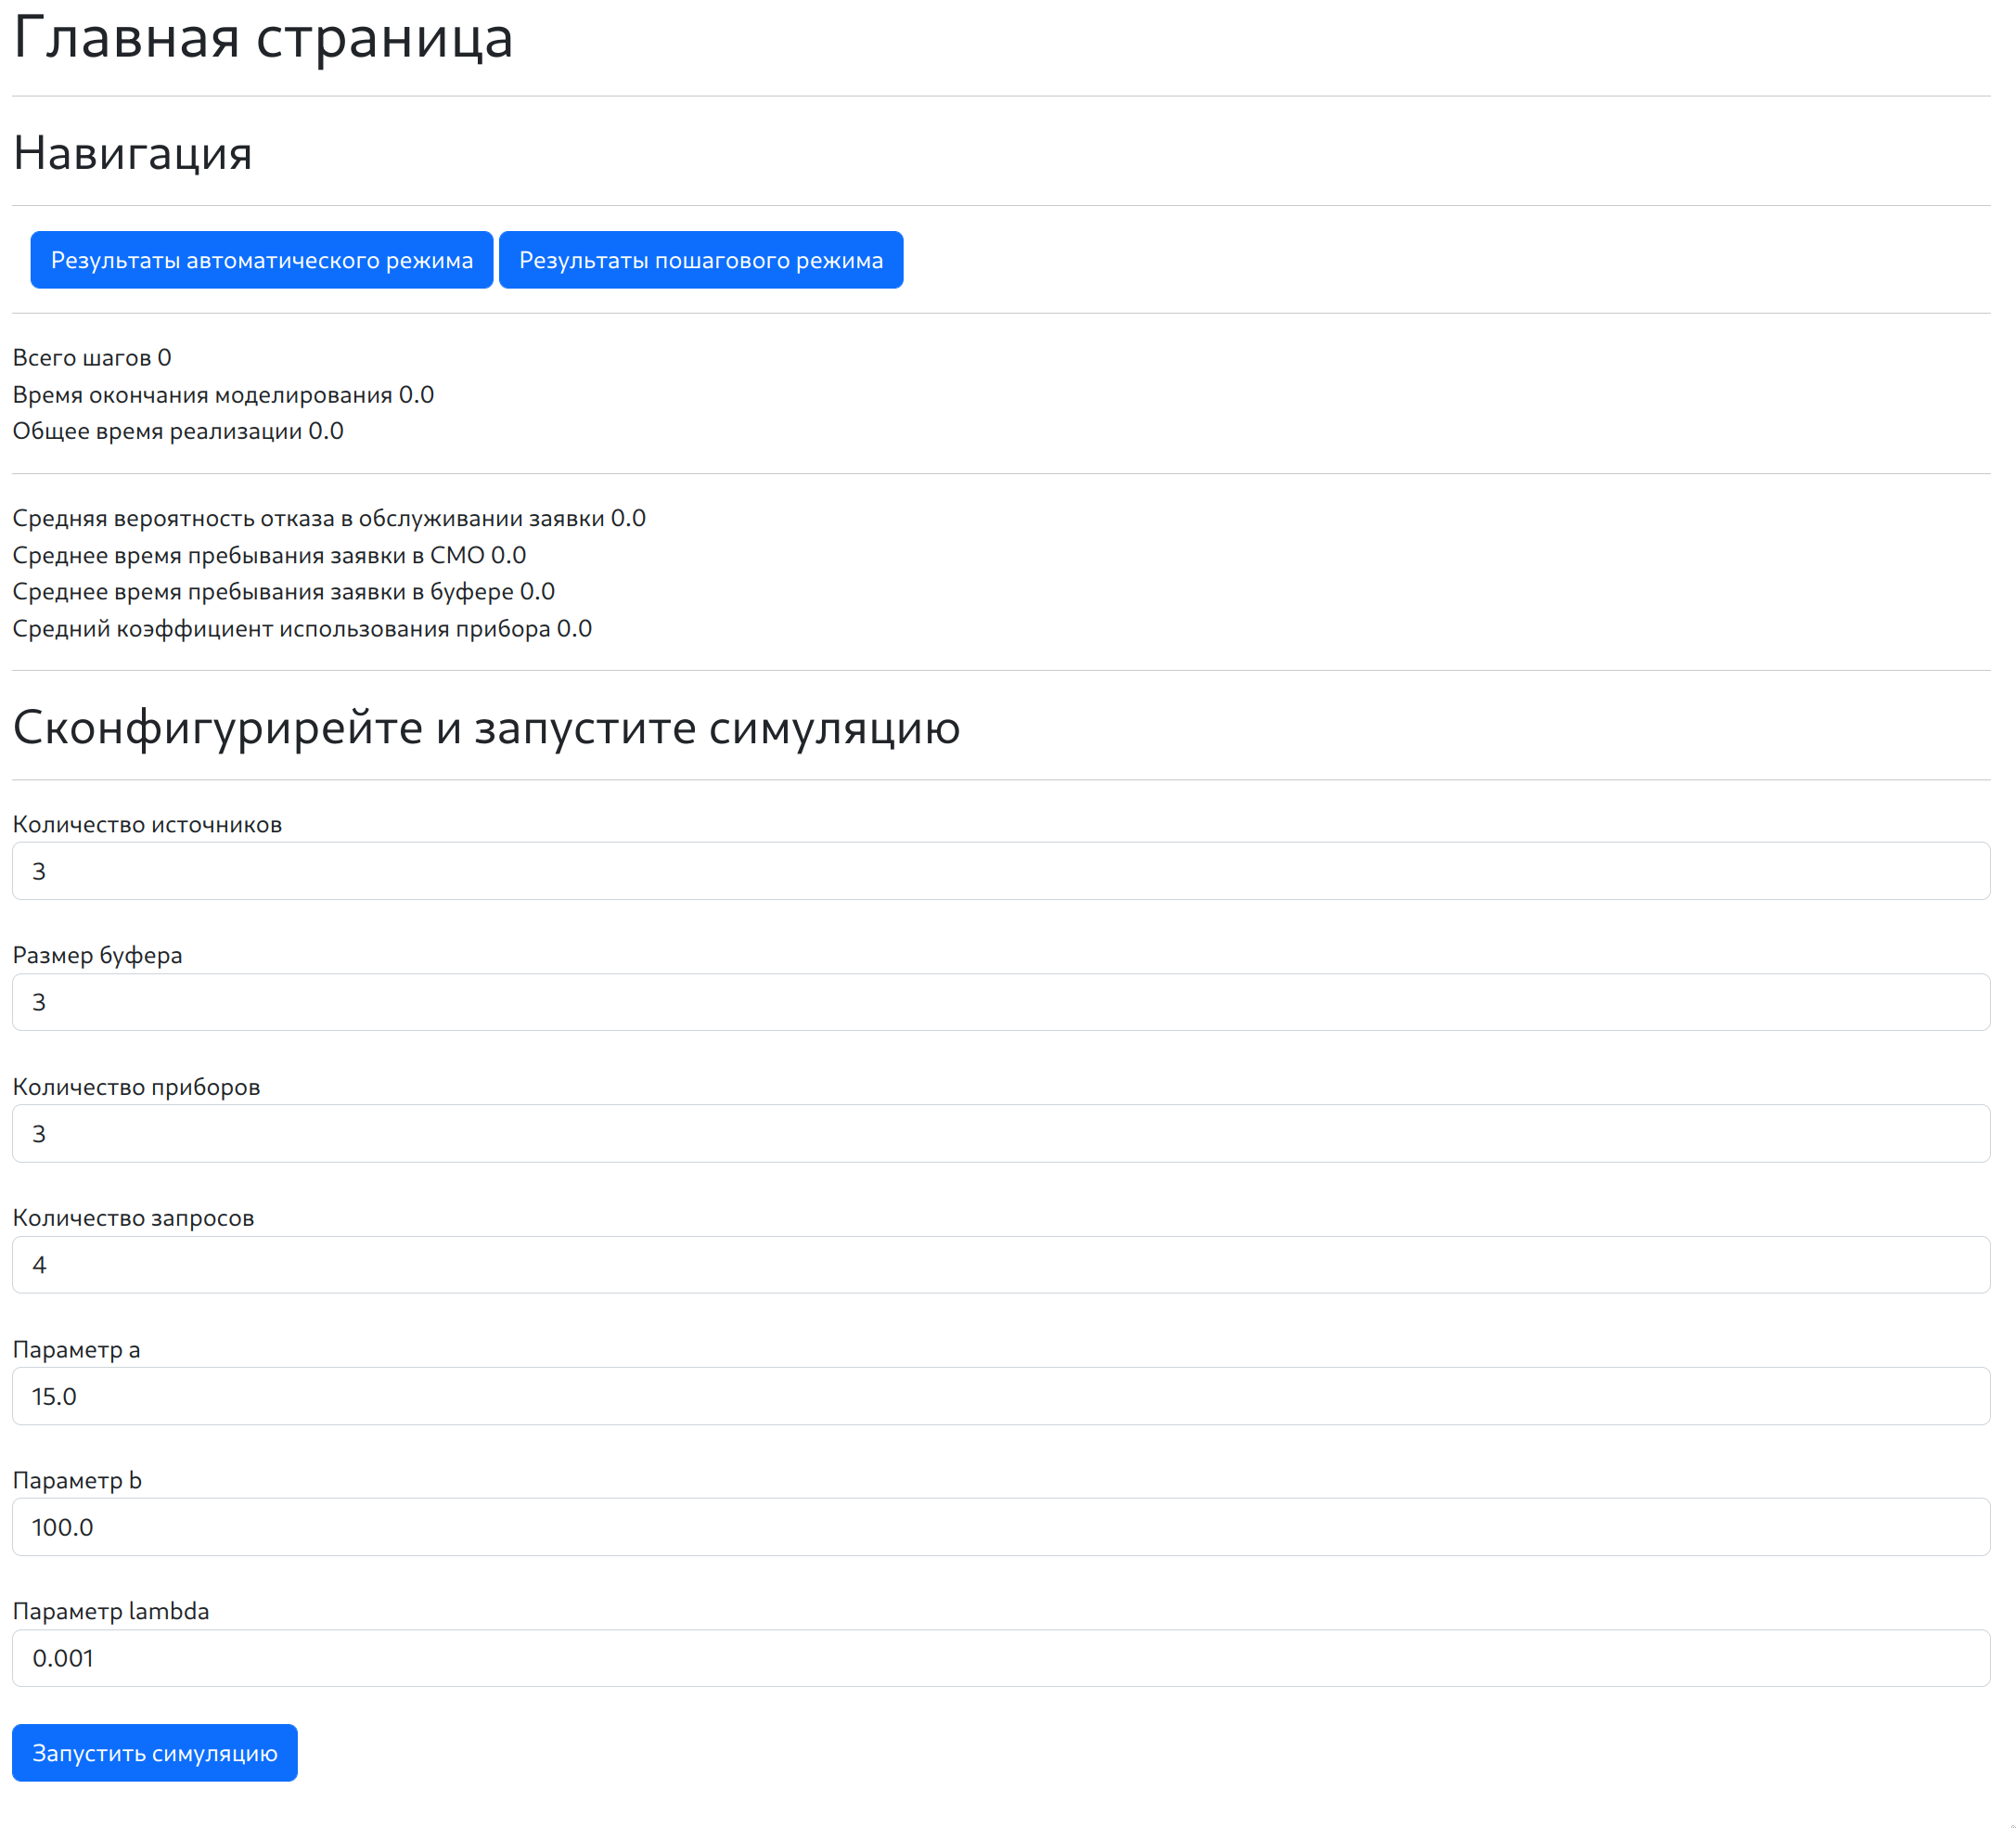
\includegraphics[width=15cm]{screenshots/1.png}\\
	\caption{Главная страница}
\end{figure}

После запуска симуляции, мы можем заметить, как отобразились результаты симуляции:

\begin{figure}[H]
	\centering
	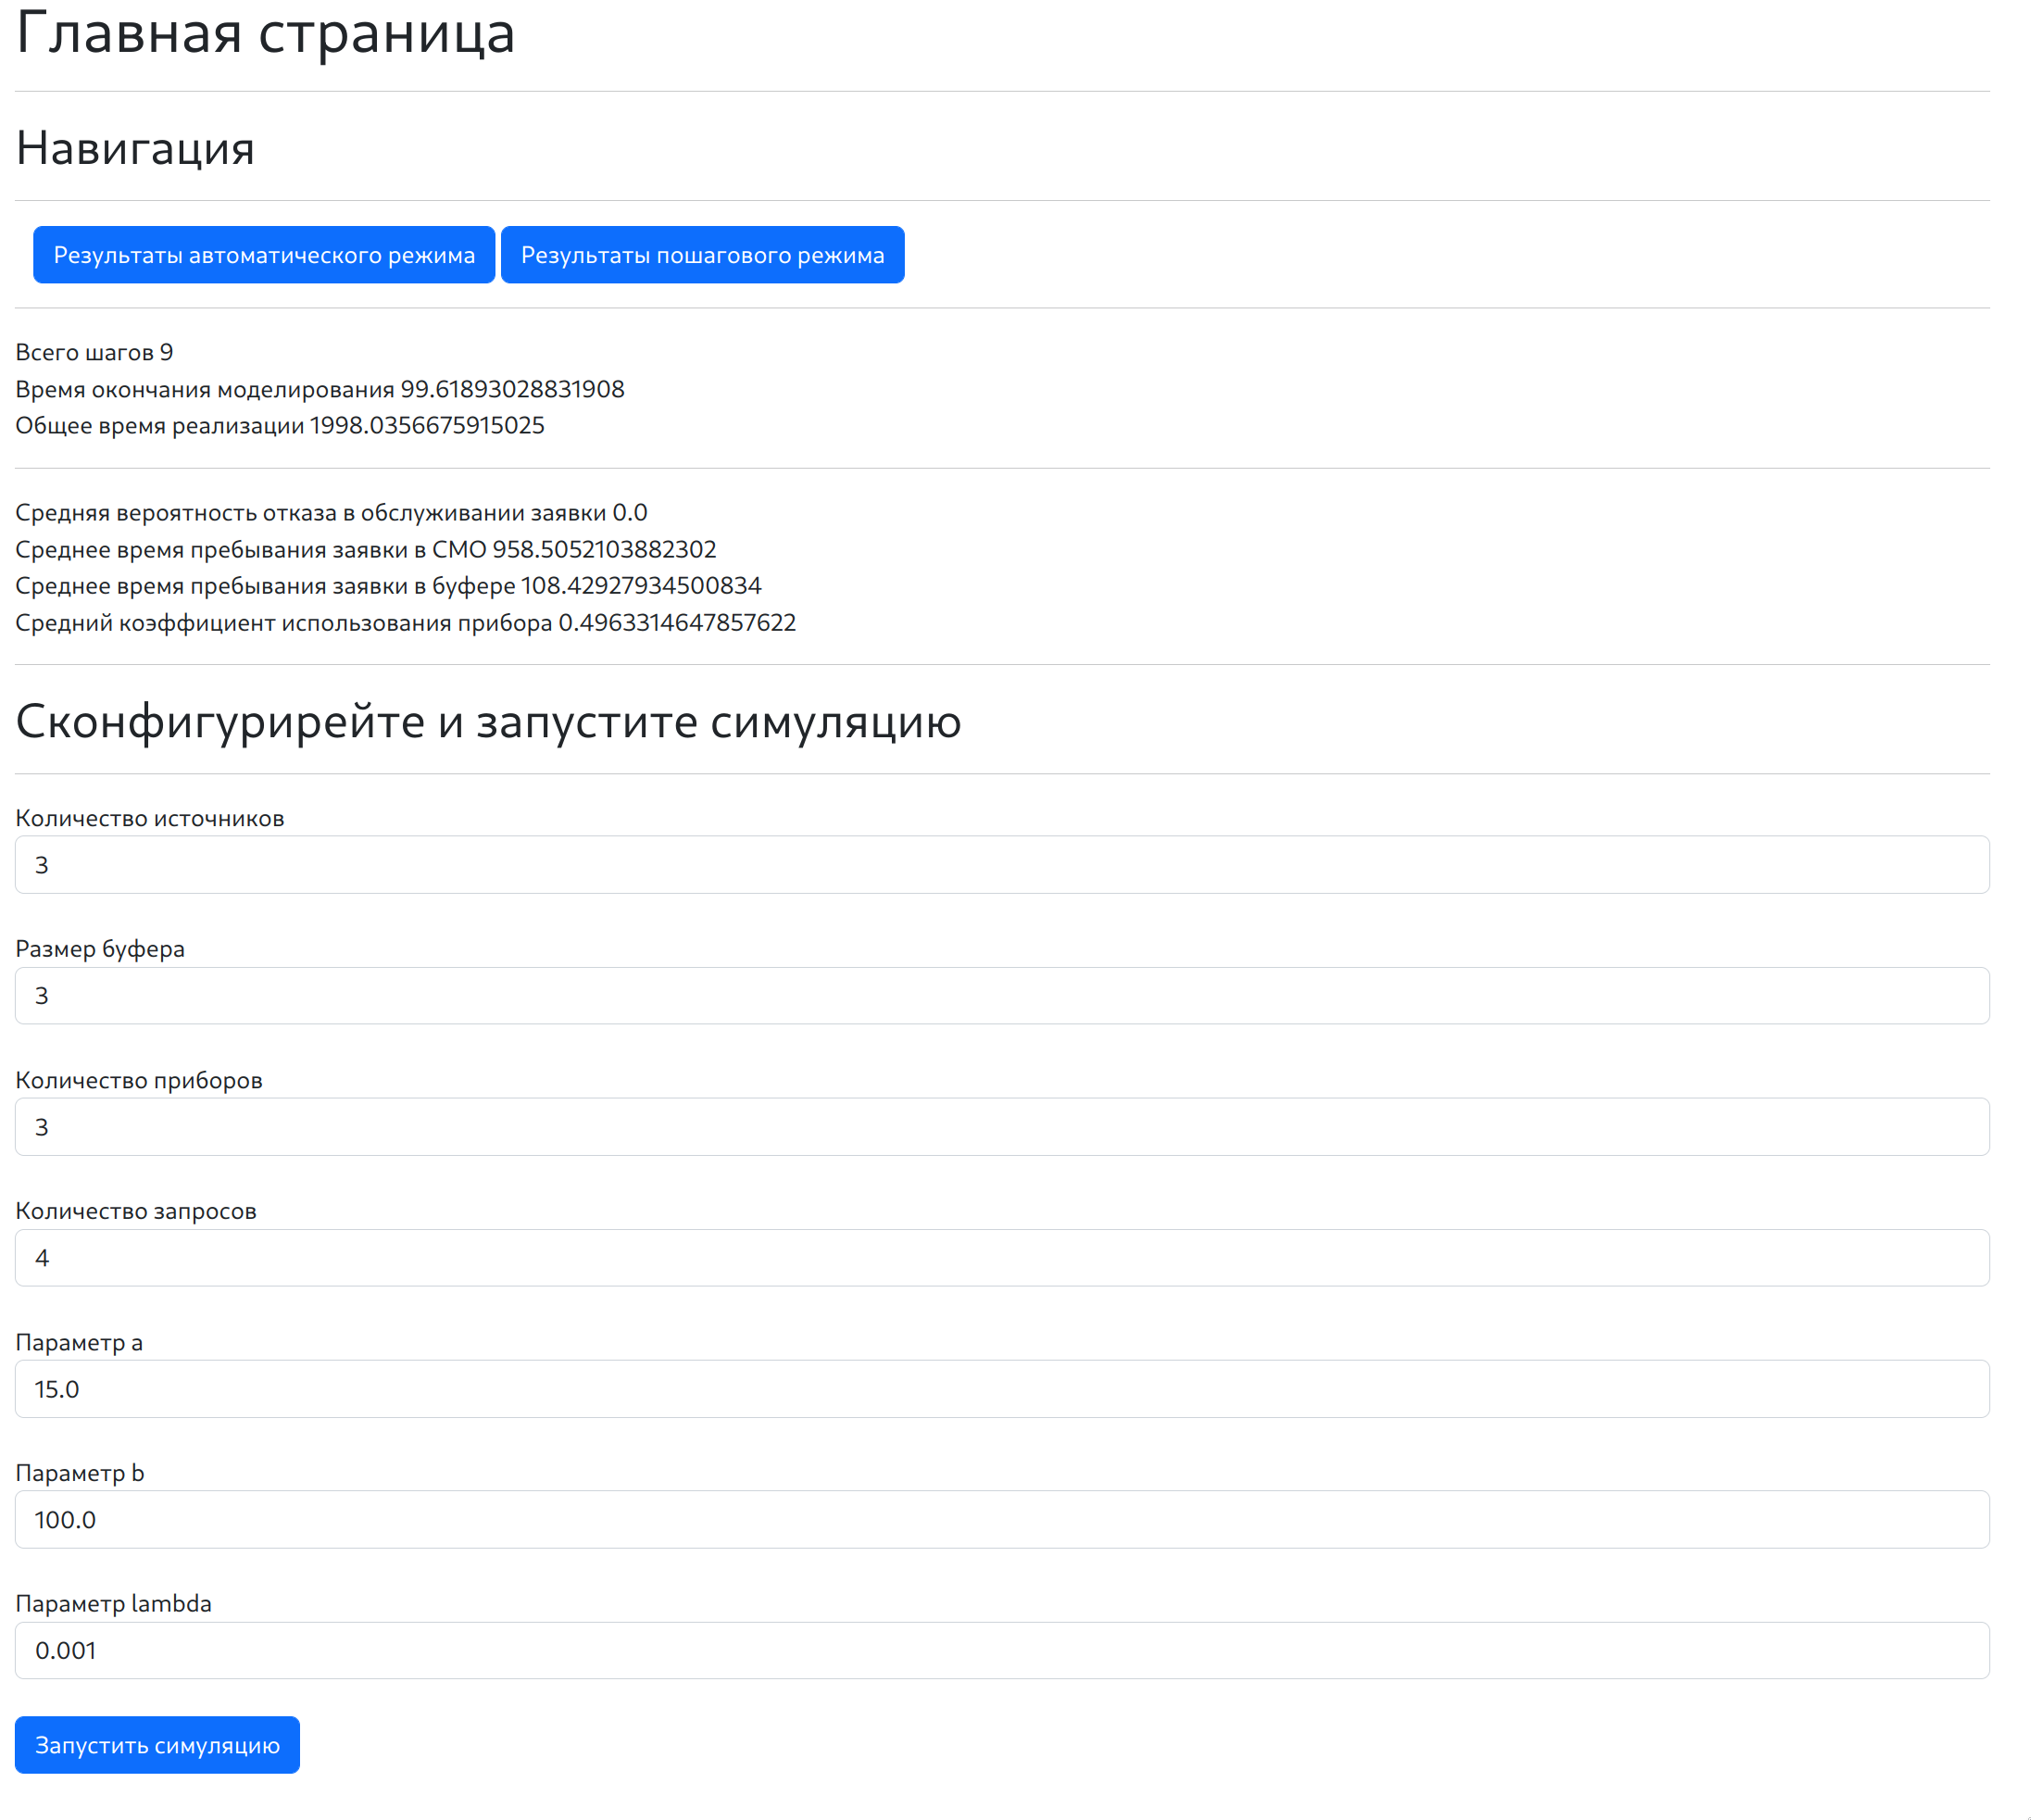
\includegraphics[width=15cm]{screenshots/2.png}\\
	\caption{Отображение результатов симуляции}
\end{figure}

Мы можем посмотреть результаты автоматического режима:

\begin{figure}[H]
	\centering
	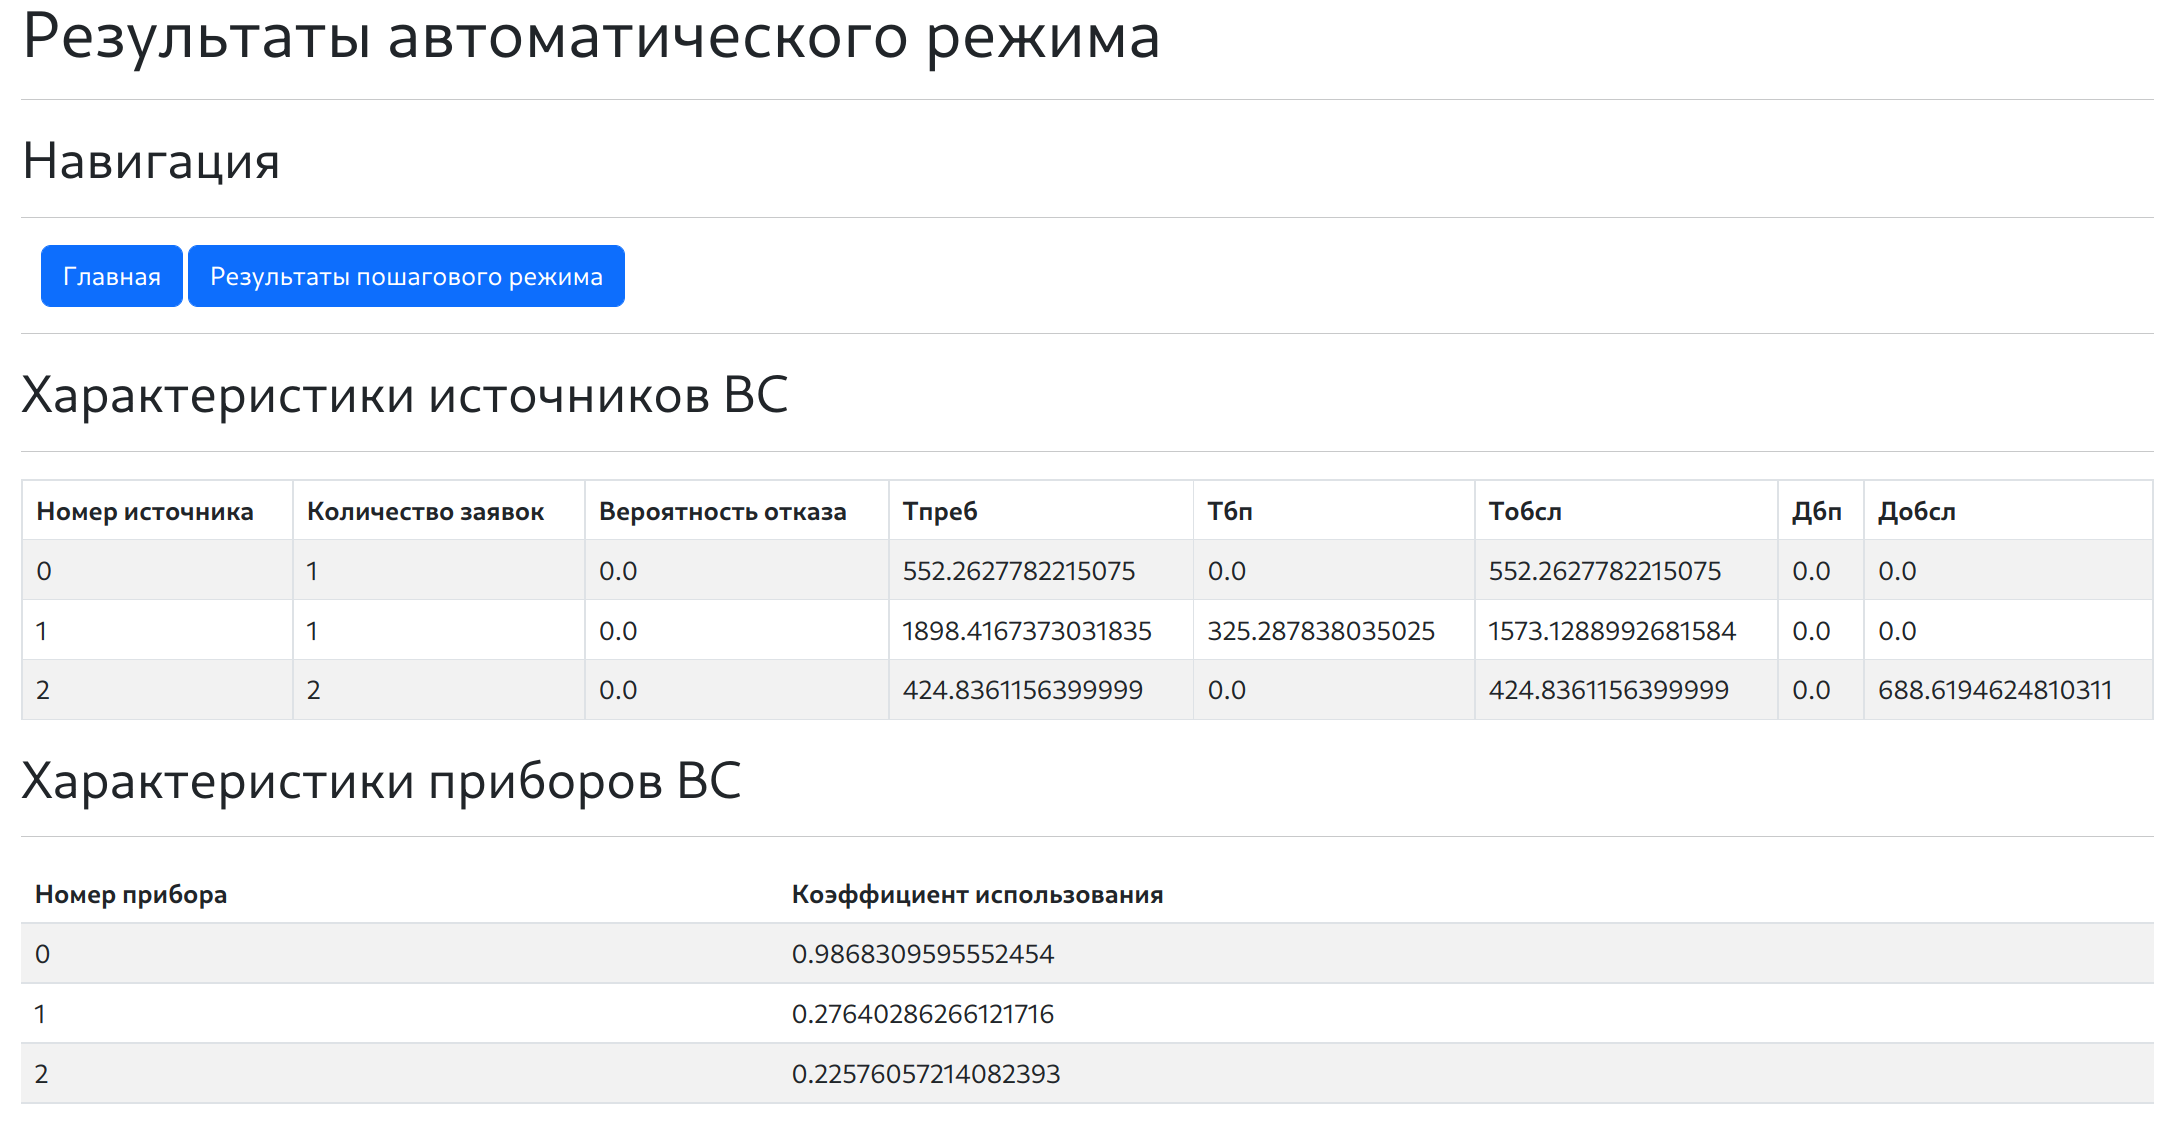
\includegraphics[width=15cm]{screenshots/3.png}\\
	\caption{Результаты автоматического режима}
\end{figure}

А также увидеть, что произошло на каждом шаге:

\begin{figure}[H]
	\centering
	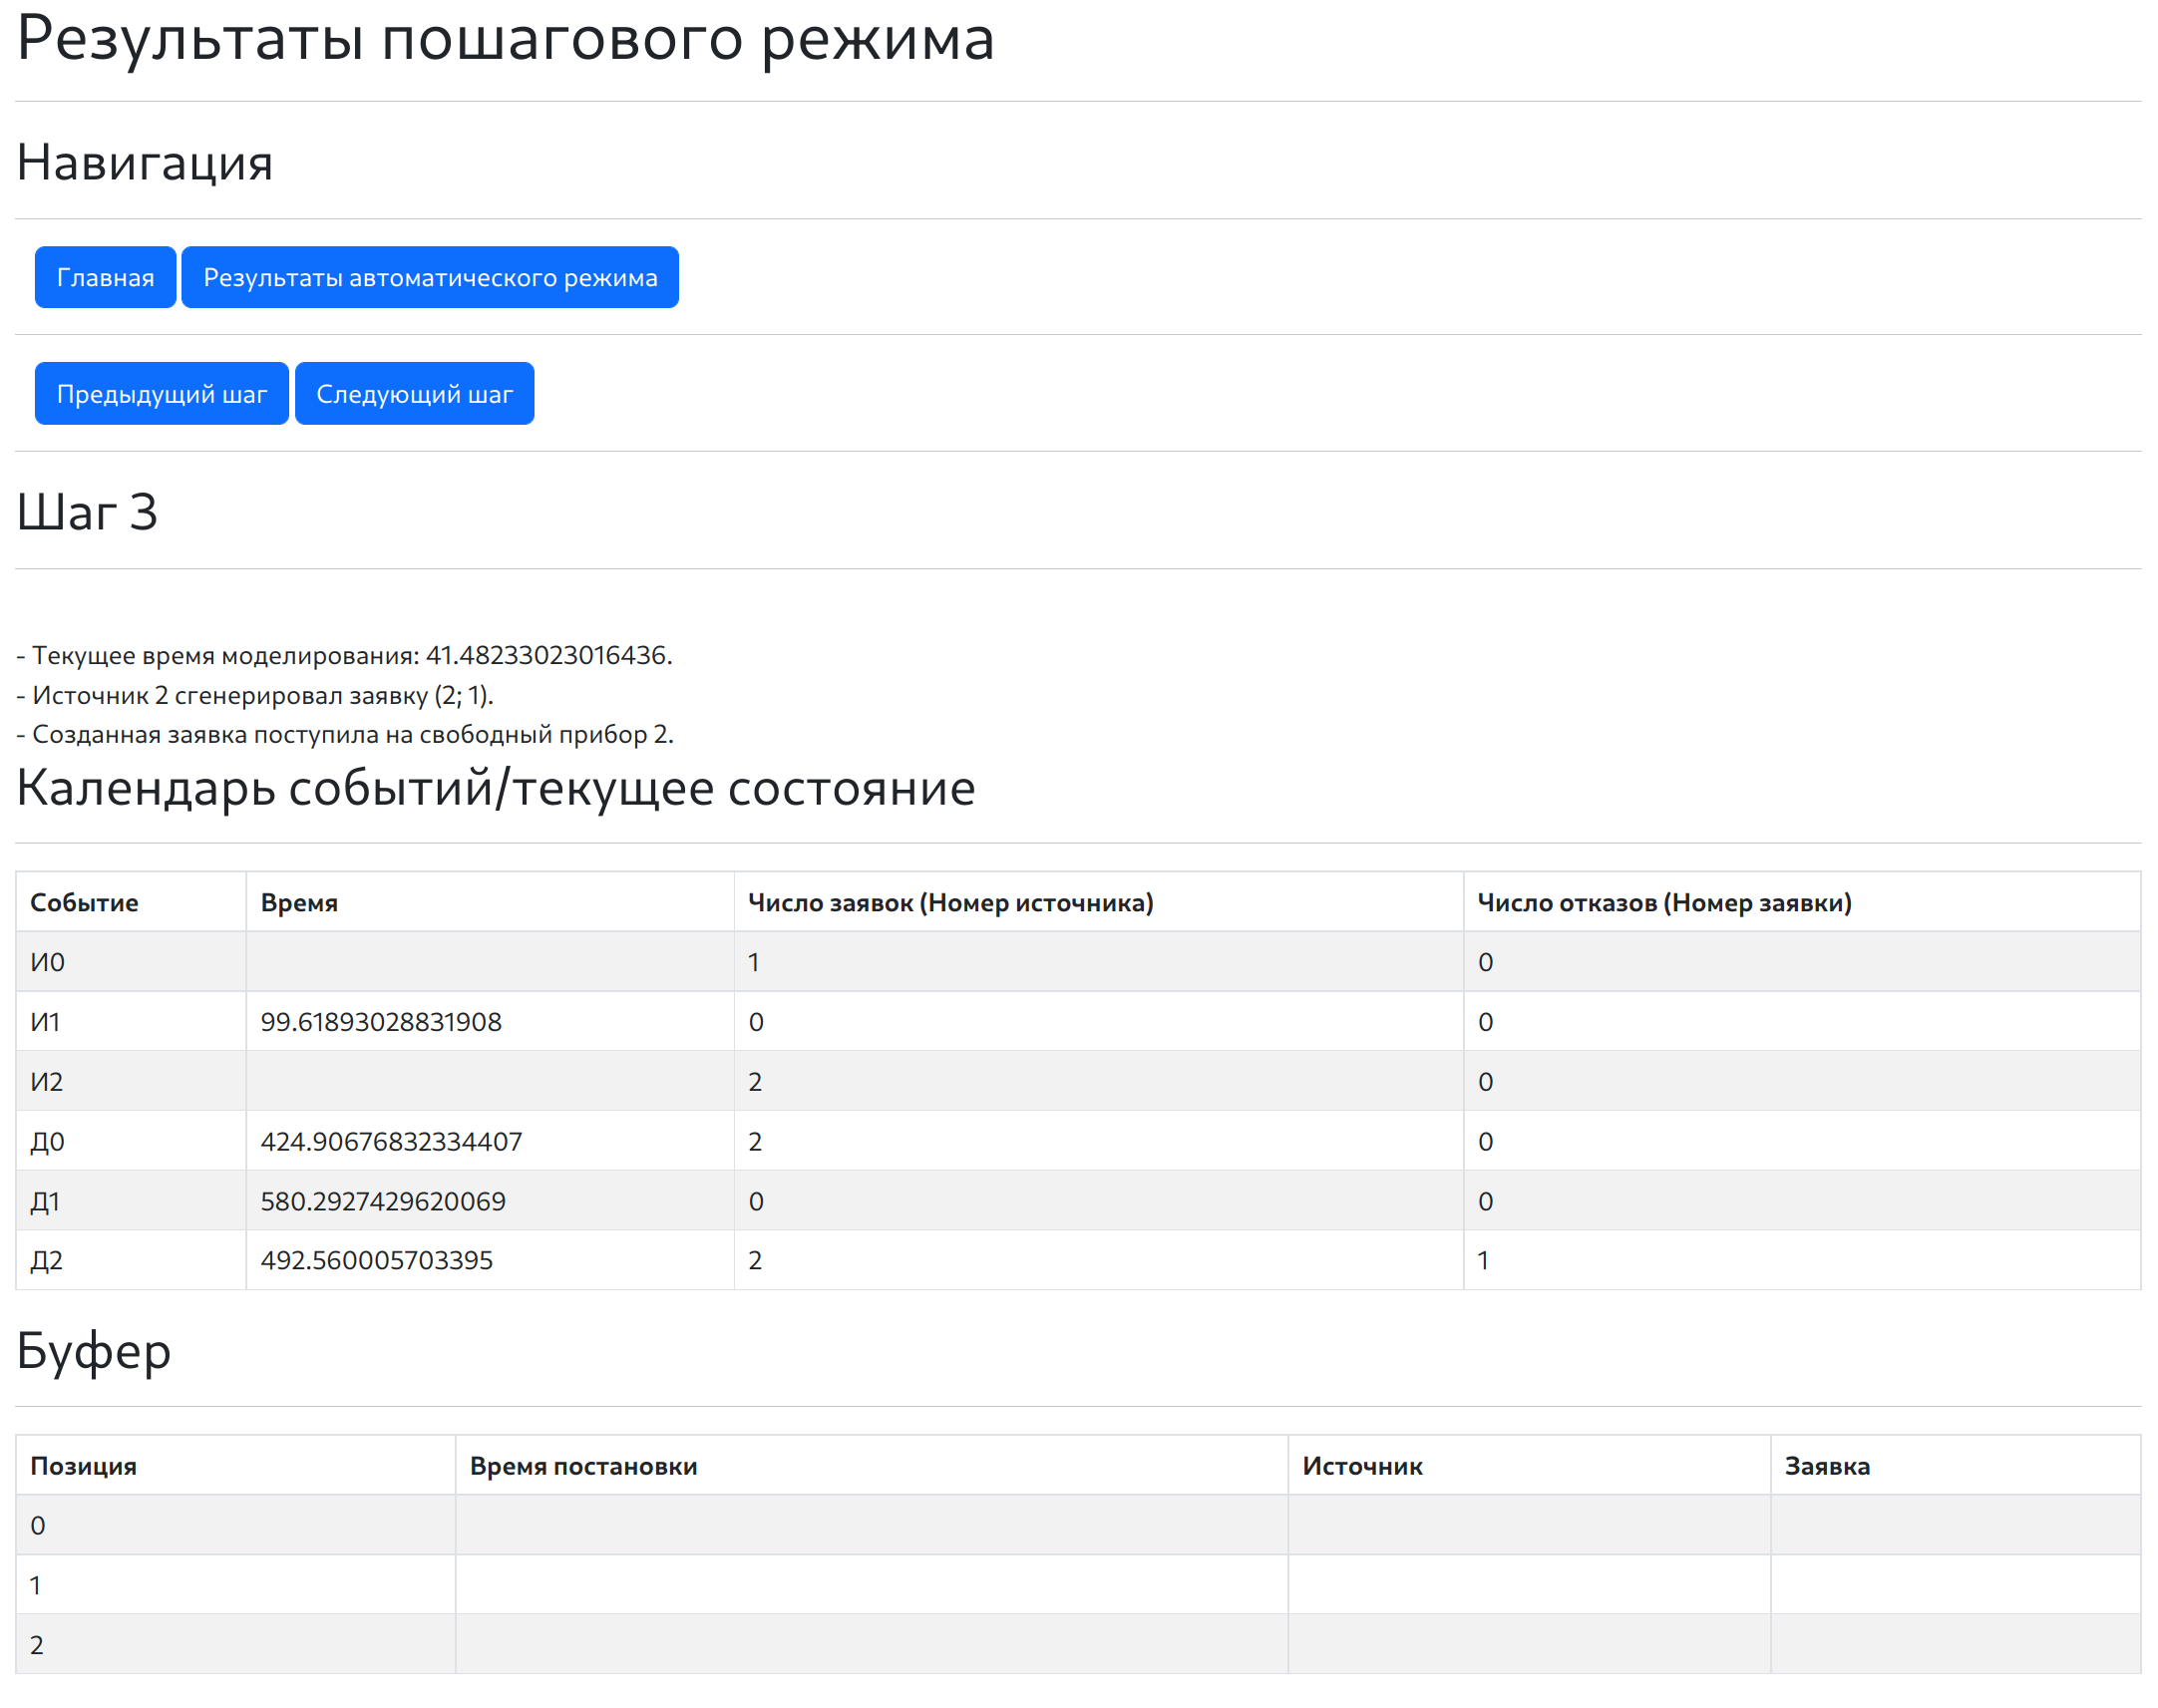
\includegraphics[width=15cm]{screenshots/4.png}\\
	\caption{Результаты пошагового режима}
\end{figure}

\section{Вывод}

По результатам курсовой работы была разработана программа для имитационного моделирования системы массового обслуживания при помощи языка \textbf{Java} и фреймворка для созданий веб-приложений \textbf{Spring}.

Посредством данной программы была проанализирована реальная система массового обслуживания, для которой были подобраны идеальные конфигурации, удовлетворяющие всем ограничениям и способные в лучшем случае повысить эффективность системы практически в \textbf{6} раз.

\end{document}